\section{Resolução Questão 17}

\begin{frame}{Questão 17}
Considere um programa de TV em que um participante deve escolher uma de três portas. Atrás de uma das portas existe um carro, enquanto nada existe atrás das outras duas.

\vspace{0.3cm}
A produção coloca o prêmio de forma aleatória atrás de uma das portas. Após a escolha de uma porta, o apresentador abre uma das outras portas que não contém o prêmio, e pergunta ao participante se ele deseja trocar sua escolha.
\end{frame}

% Slide 2: Portas
\begin{frame}{Qual porta escolher?}
\centering
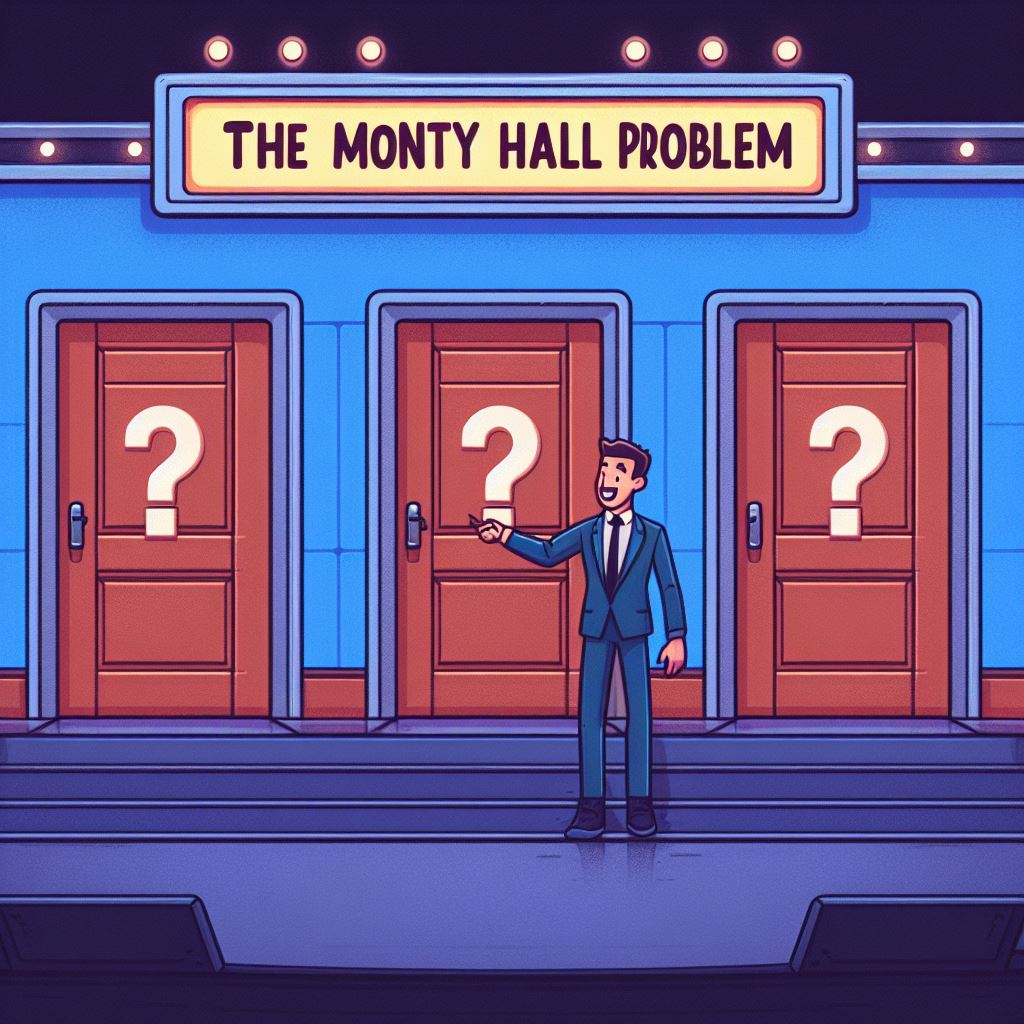
\includegraphics[width=0.45\textwidth]{figures/MontyHall.jpeg}
\end{frame}

% Slide 3: Código
\begin{frame}[fragile]{Simulação}
 \begin{figure}
    \centering
    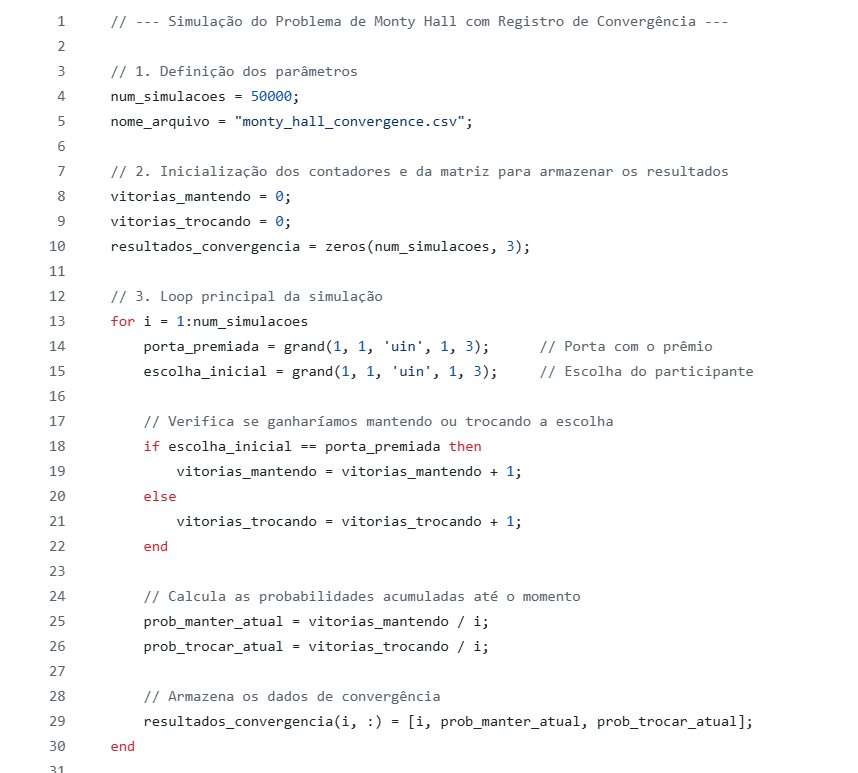
\includegraphics[width=0.9\linewidth]{figures/Captura de tela 2025-07-18 154707.png}
 \end{figure}
\end{frame}

\begin{frame}[fragile]{Simulação}
 \begin{figure}
    \centering
    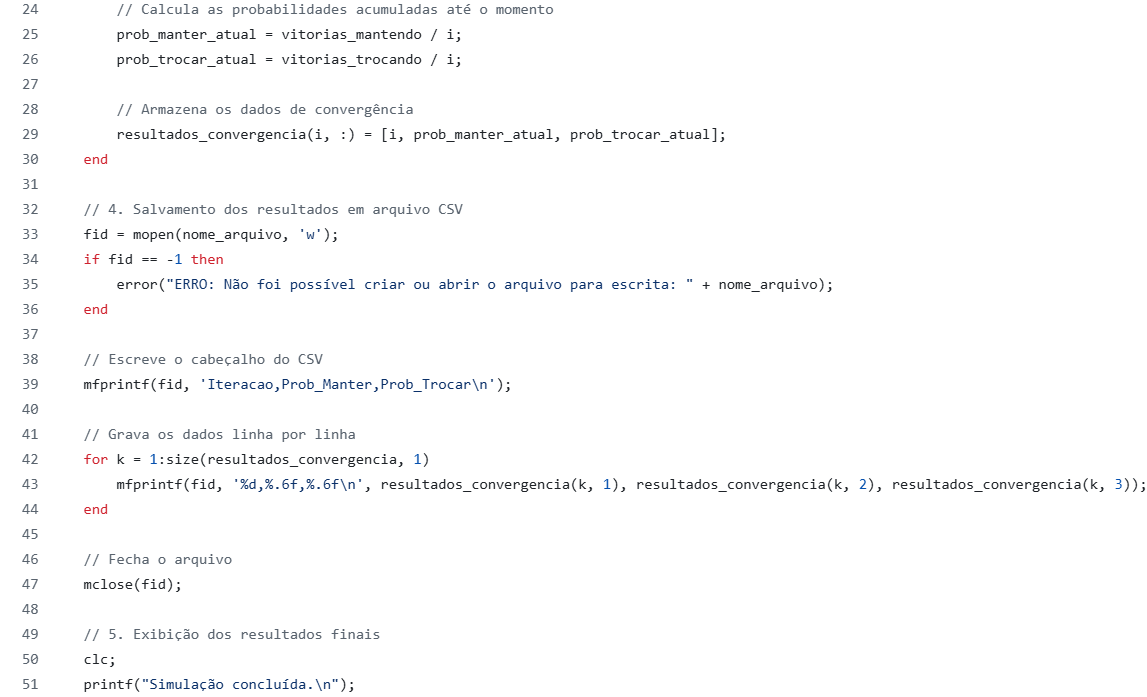
\includegraphics[width=0.9\linewidth]{figures/parte ok 2.png}
 \end{figure}
\end{frame}

\begin{frame}[fragile]{Simulação}
 \begin{figure}
    \centering
    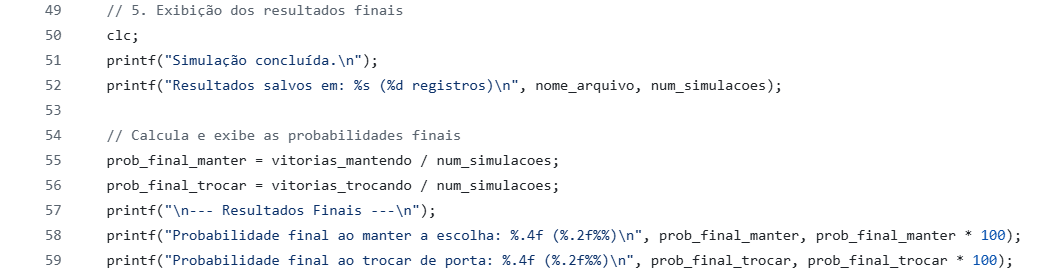
\includegraphics[width=0.9\linewidth]{figures/Captura de tela 2025-07-18 160019.png}
 \end{figure}
\end{frame}

\begin{frame}[fragile]{Convergência}
 \begin{figure}
    \centering
    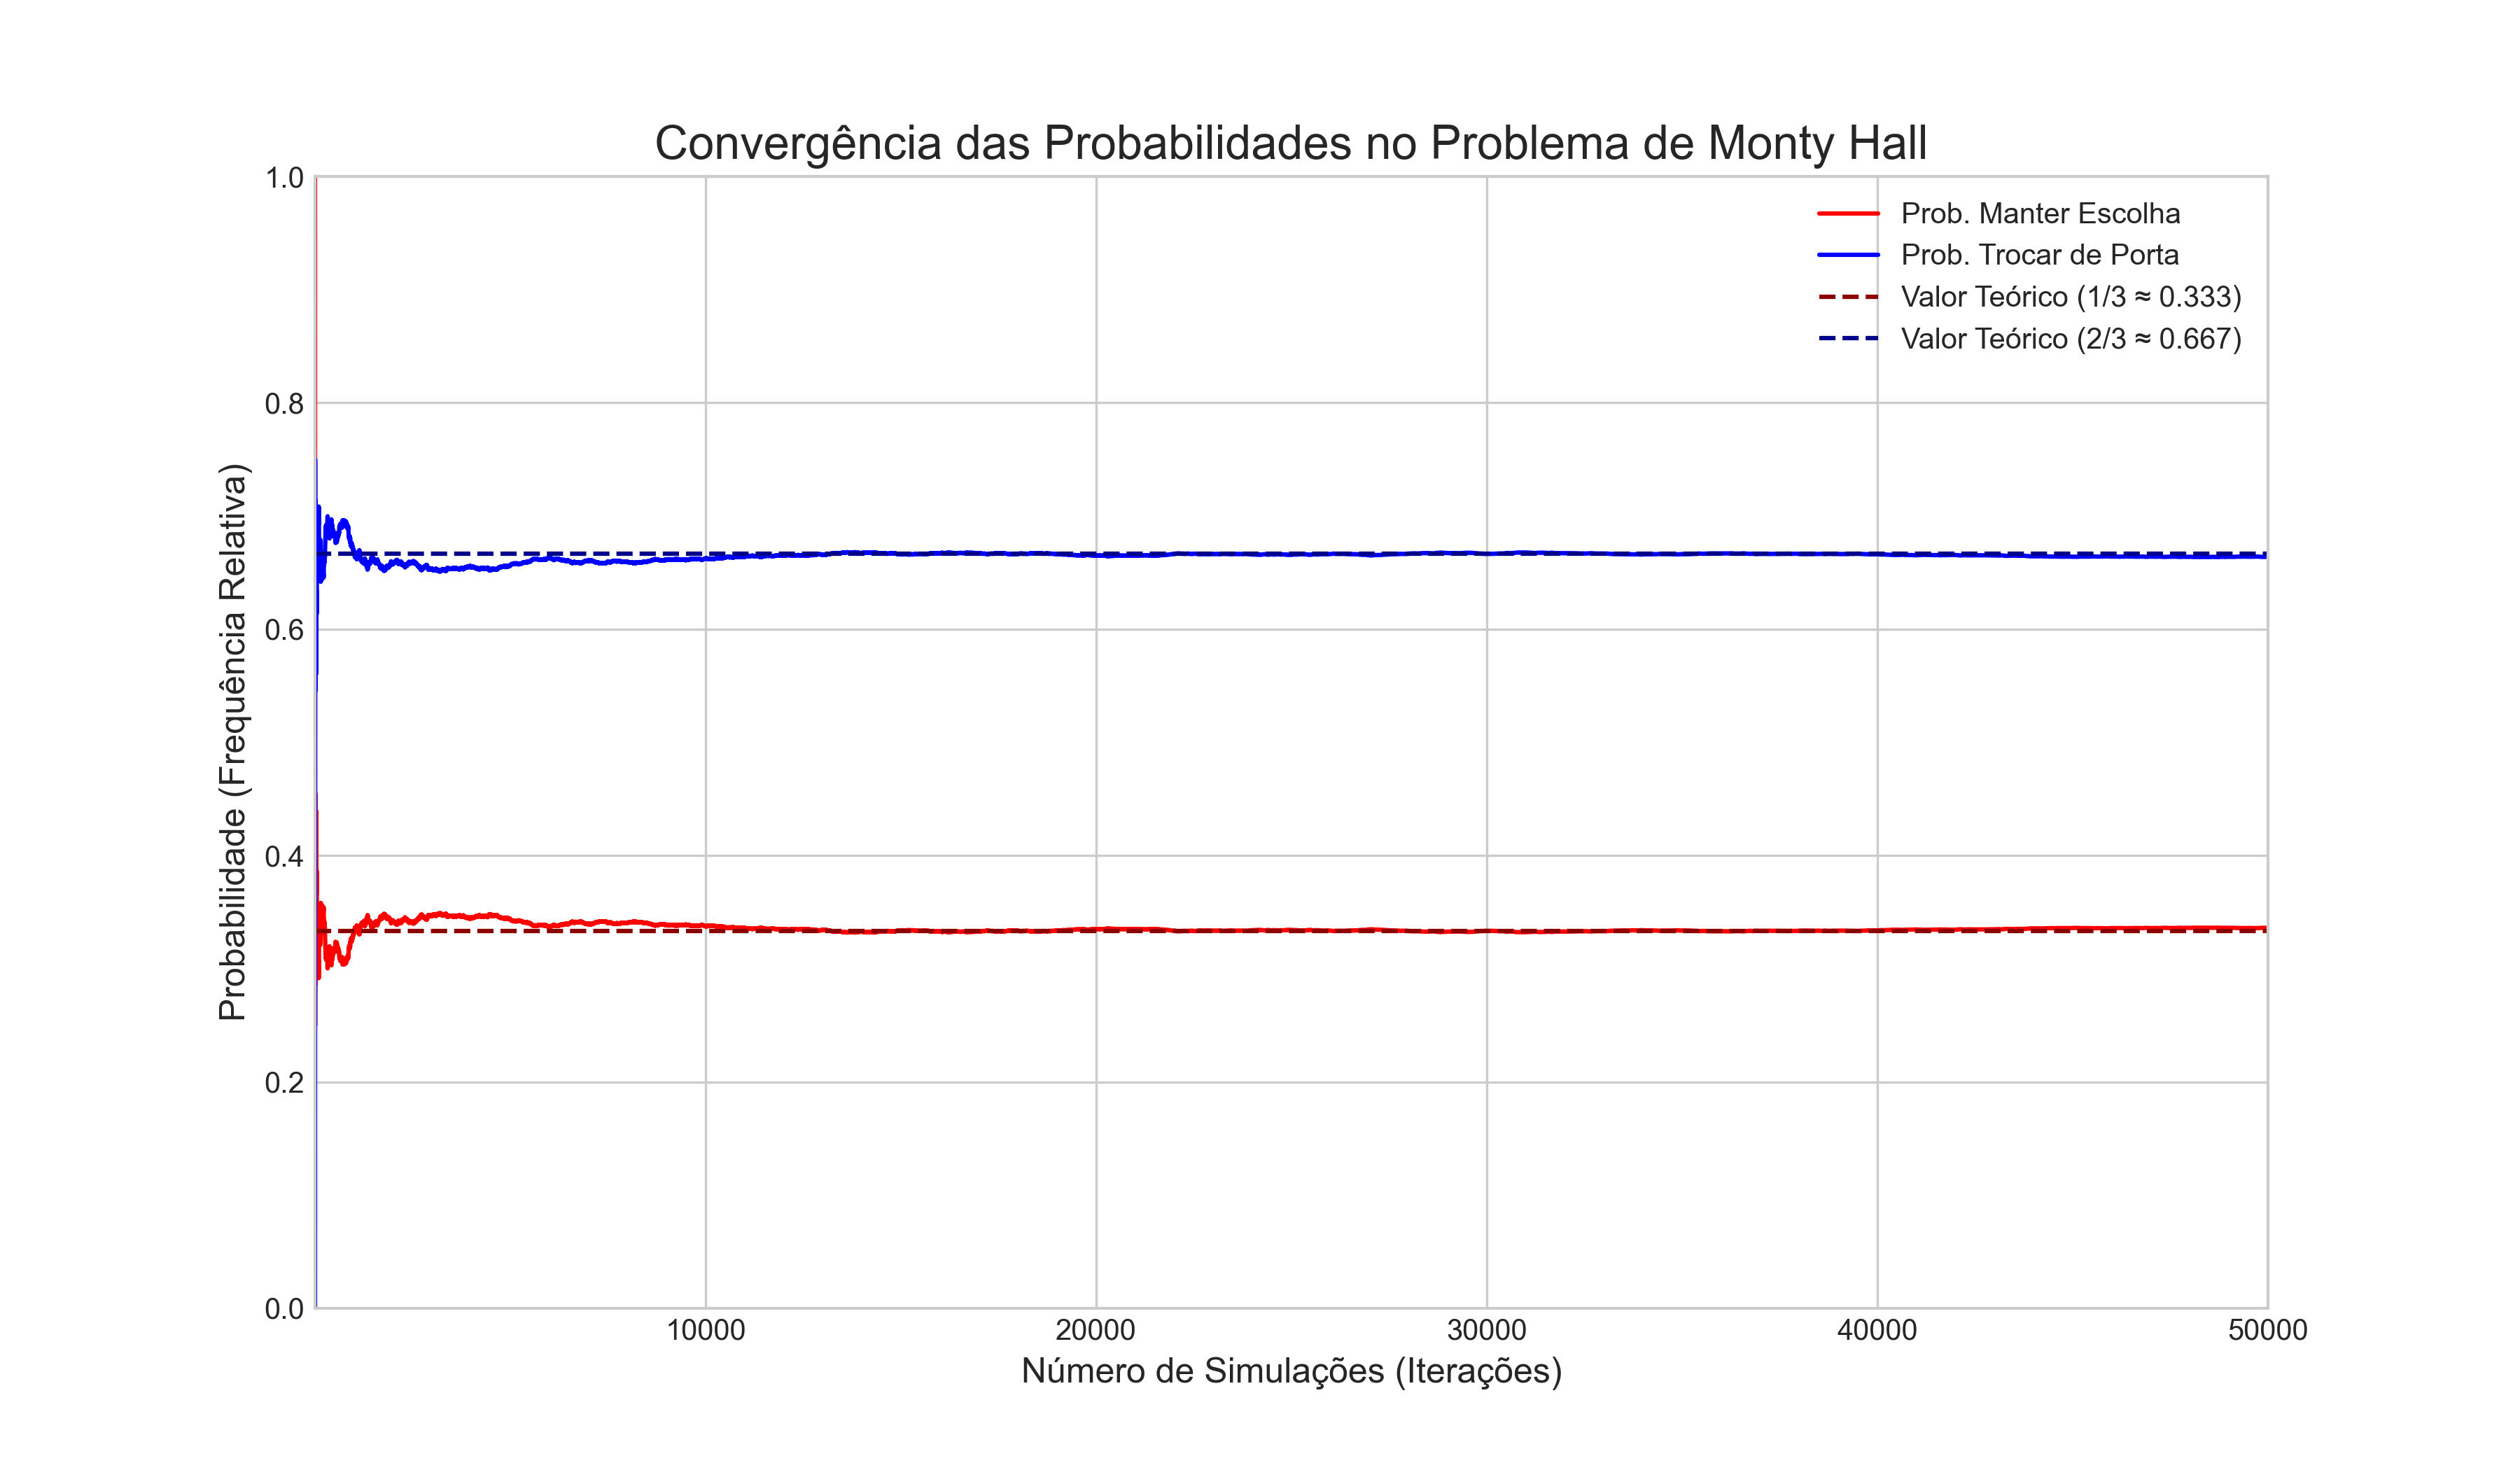
\includegraphics[width=0.9\linewidth]{figures/convergencia_monty_hall.png}
 \end{figure}
\end{frame}

% Slide 5: Código - Trocando
\begin{frame}[fragile]{Sempre trocando de porta}
A resposta intuitiva ao problema é a que quando o apresentador revelou uma das portas não premiadas, o participante passaria a ter um novo dilema com duas portas e um prêmio. Portanto, a chance do prêmio estar em uma das portas seria 1/2. 
 
A resposta contra-intuitiva e certa é que é mais vantajoso trocar, pois a
chance de ganhar trocando é o dobro da chance de ganhar sem trocar
\begin{figure}
    \centering
    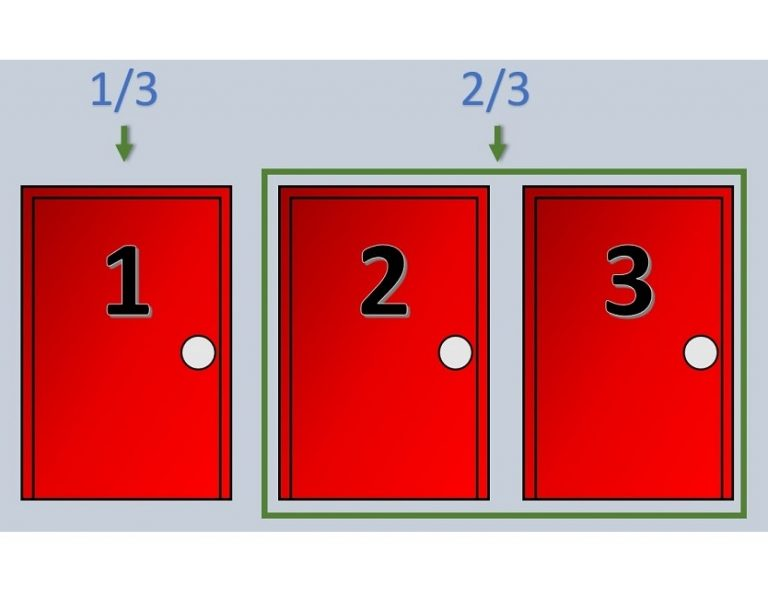
\includegraphics[width=0.45\linewidth]{figures/porc portas.jpg}
    \label{fig:enter-label}
 \end{figure}
\end{frame}
% Slide 6: Resultado
\begin{frame}{Solução}
\textbf{Resposta correta: é melhor trocar de porta!}

\vspace{0.3cm}
\begin{itemize}
  \item Probabilidade de ganhar sem trocar: \textbf{1/3}
  \item Probabilidade de ganhar trocando: \textbf{2/3}
\end{itemize}

\vspace{0.4cm}
\centering
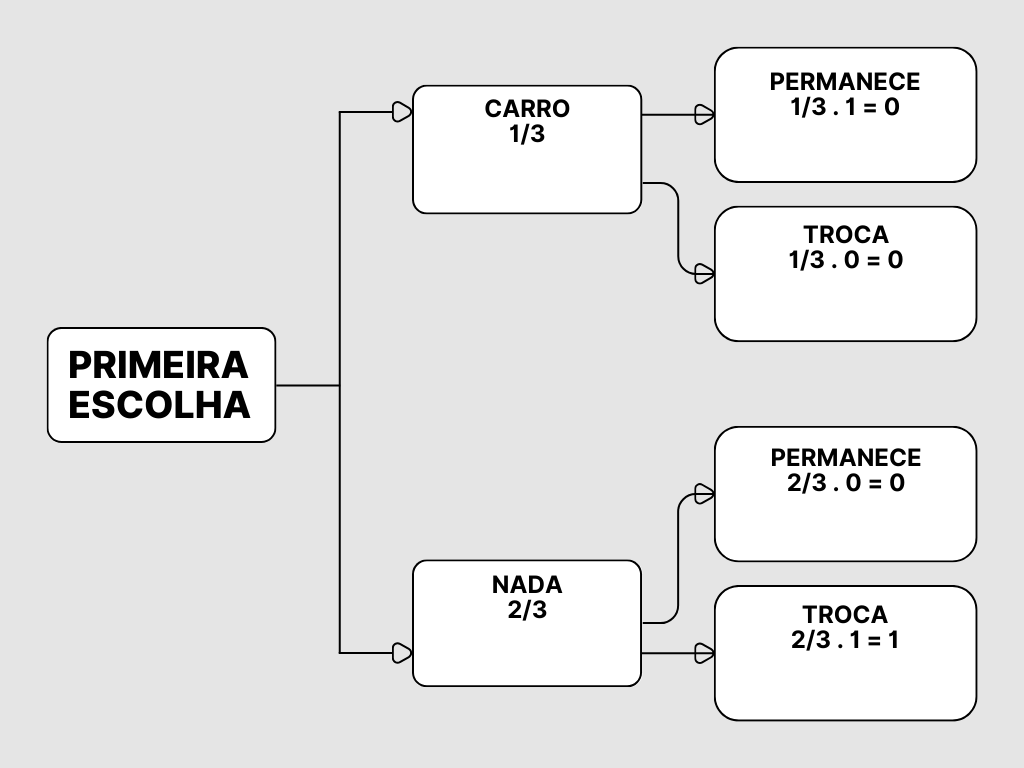
\includegraphics[width=0.4\textwidth]{figures/Grey and White Minimalist Simple Concept Map.png} 
\end{frame}